\documentclass[tikz,border=6pt]{standalone}
% Shared visual language for the original benchmark atlas.
\usepackage[T1]{fontenc}
\usepackage{lmodern}
\usepackage{amsmath,amssymb}
\usetikzlibrary{arrows.meta,calc,positioning,shapes.geometric,patterns,decorations.pathmorphing,backgrounds,fit}
\definecolor{ink}{HTML}{173948}
\definecolor{flow}{HTML}{167D9A}
\definecolor{control}{HTML}{A65217}
\definecolor{measure}{HTML}{70518A}
\definecolor{pale}{HTML}{EAF2F5}
\definecolor{muted}{HTML}{526571}
\definecolor{utility}{HTML}{2E8665}
\tikzset{
  every node/.style={font=\sffamily\small,text=ink},
  equipment/.style={draw=ink,line width=1pt,fill=pale,rounded corners=2pt},
  process/.style={draw=flow,line width=1.2pt,-{Latex[length=2.5mm]}},
  signal/.style={draw=control,line width=.8pt,dashed,-{Latex[length=2mm]}},
  util/.style={draw=utility,line width=1pt,-{Latex[length=2.2mm]}},
  dimension/.style={draw=muted,line width=.6pt,{Latex[length=1.7mm]}-{Latex[length=1.7mm]}},
  labelbox/.style={fill=white,inner sep=2pt,font=\sffamily\footnotesize,align=center},
  annotation/.style={font=\sffamily\footnotesize,text=muted,align=left},
  panel/.style={draw=ink!20,fill=ink!2,rounded corners=3pt,inner sep=6pt},
  instrument/.style={circle,draw=measure,fill=white,line width=.8pt,minimum size=8mm,inner sep=1pt,font=\sffamily\scriptsize,align=center},
  port/.style={circle,fill=flow,inner sep=1.6pt},
  box/.style={equipment,minimum width=3cm,minimum height=1cm,align=center},
}
\newcommand{\atlasheader}[3]{%
  \node[anchor=north west,font=\sffamily\bfseries\LARGE] at (0,0) {#1};%
  \node[anchor=north west,font=\sffamily\small,text=muted] at (0,-.75) {Paper section #2: \textit{#3}};%
  \draw[ink!25,line width=.7pt] (0,-1.25)--(26,-1.25);%
}
\newcommand{\atlasfooter}[1]{%
  \draw[ink!25,line width=.5pt] (0,-15.8)--(26,-15.8);%
  \node[anchor=north west,annotation,text width=25.8cm] at (0,-16) {#1\\Original explanatory drawing. Source: Kroll \& Schulte (2014), DOI: 10.1016/j.asoc.2014.08.034. Model variants are identified in the accompanying case sheet.};%
}

\usetikzlibrary{shadings,shadows,decorations.markings}
% Figure 4 of Schulte--Hahn as reproduced in the Kroll--Schulte survey,
% interpreted as a colored engineering illustration. Functional topology is
% the reference; metal surfaces and test-cell scenery are illustrative only.
% The surveyed local deviation model and the distinct physical SI teaching
% model are not silently equated with an instrumented original apparatus.
\definecolor{wallWarm}{HTML}{F4F1E9}
\definecolor{wallCool}{HTML}{E0EAEB}
\definecolor{dayLight}{HTML}{F7E8C9}
\definecolor{metalDark}{HTML}{50656F}
\definecolor{metalMid}{HTML}{A8BCC2}
\definecolor{metalLight}{HTML}{F2F3EA}
\definecolor{metalBlue}{HTML}{64899B}
\definecolor{metalDeep}{HTML}{2F5368}
\definecolor{warmBrass}{HTML}{BE9567}
\definecolor{warmCopper}{HTML}{C1875C}
\definecolor{copperDeep}{HTML}{805C47}
\definecolor{chamberTwo}{HTML}{DCEAEC}
\definecolor{chamberOne}{HTML}{E8EDE5}
\definecolor{airBlue}{HTML}{267FA7}
\definecolor{airLight}{HTML}{9FD8E1}
\definecolor{supply}{HTML}{BB8745}
\definecolor{returnFlow}{HTML}{57899B}
\definecolor{signalPurple}{HTML}{755B9D}
\definecolor{guide}{HTML}{71838B}
\tikzset{
  subtlelabel/.style={font=\sffamily\footnotesize,text=ink,align=center,inner sep=0pt},
  smalllabel/.style={font=\sffamily\scriptsize,text=ink,inner sep=0pt,align=center},
  portarrow/.style={line width=1.02pt,-{Stealth[length=2.12mm,width=1.45mm]},line cap=round},
  pointer/.style={draw=guide!75,line width=.60pt,-{Stealth[length=1.65mm,width=1.1mm]},line cap=round},
  forcearrow/.style={draw=copperDeep,line width=1.10pt,-{Stealth[length=2.40mm,width=1.68mm]},line cap=round},
  labpanel/.style={panel,draw=metalDark!23,fill=wallCool!45!white},
}
\begin{document}
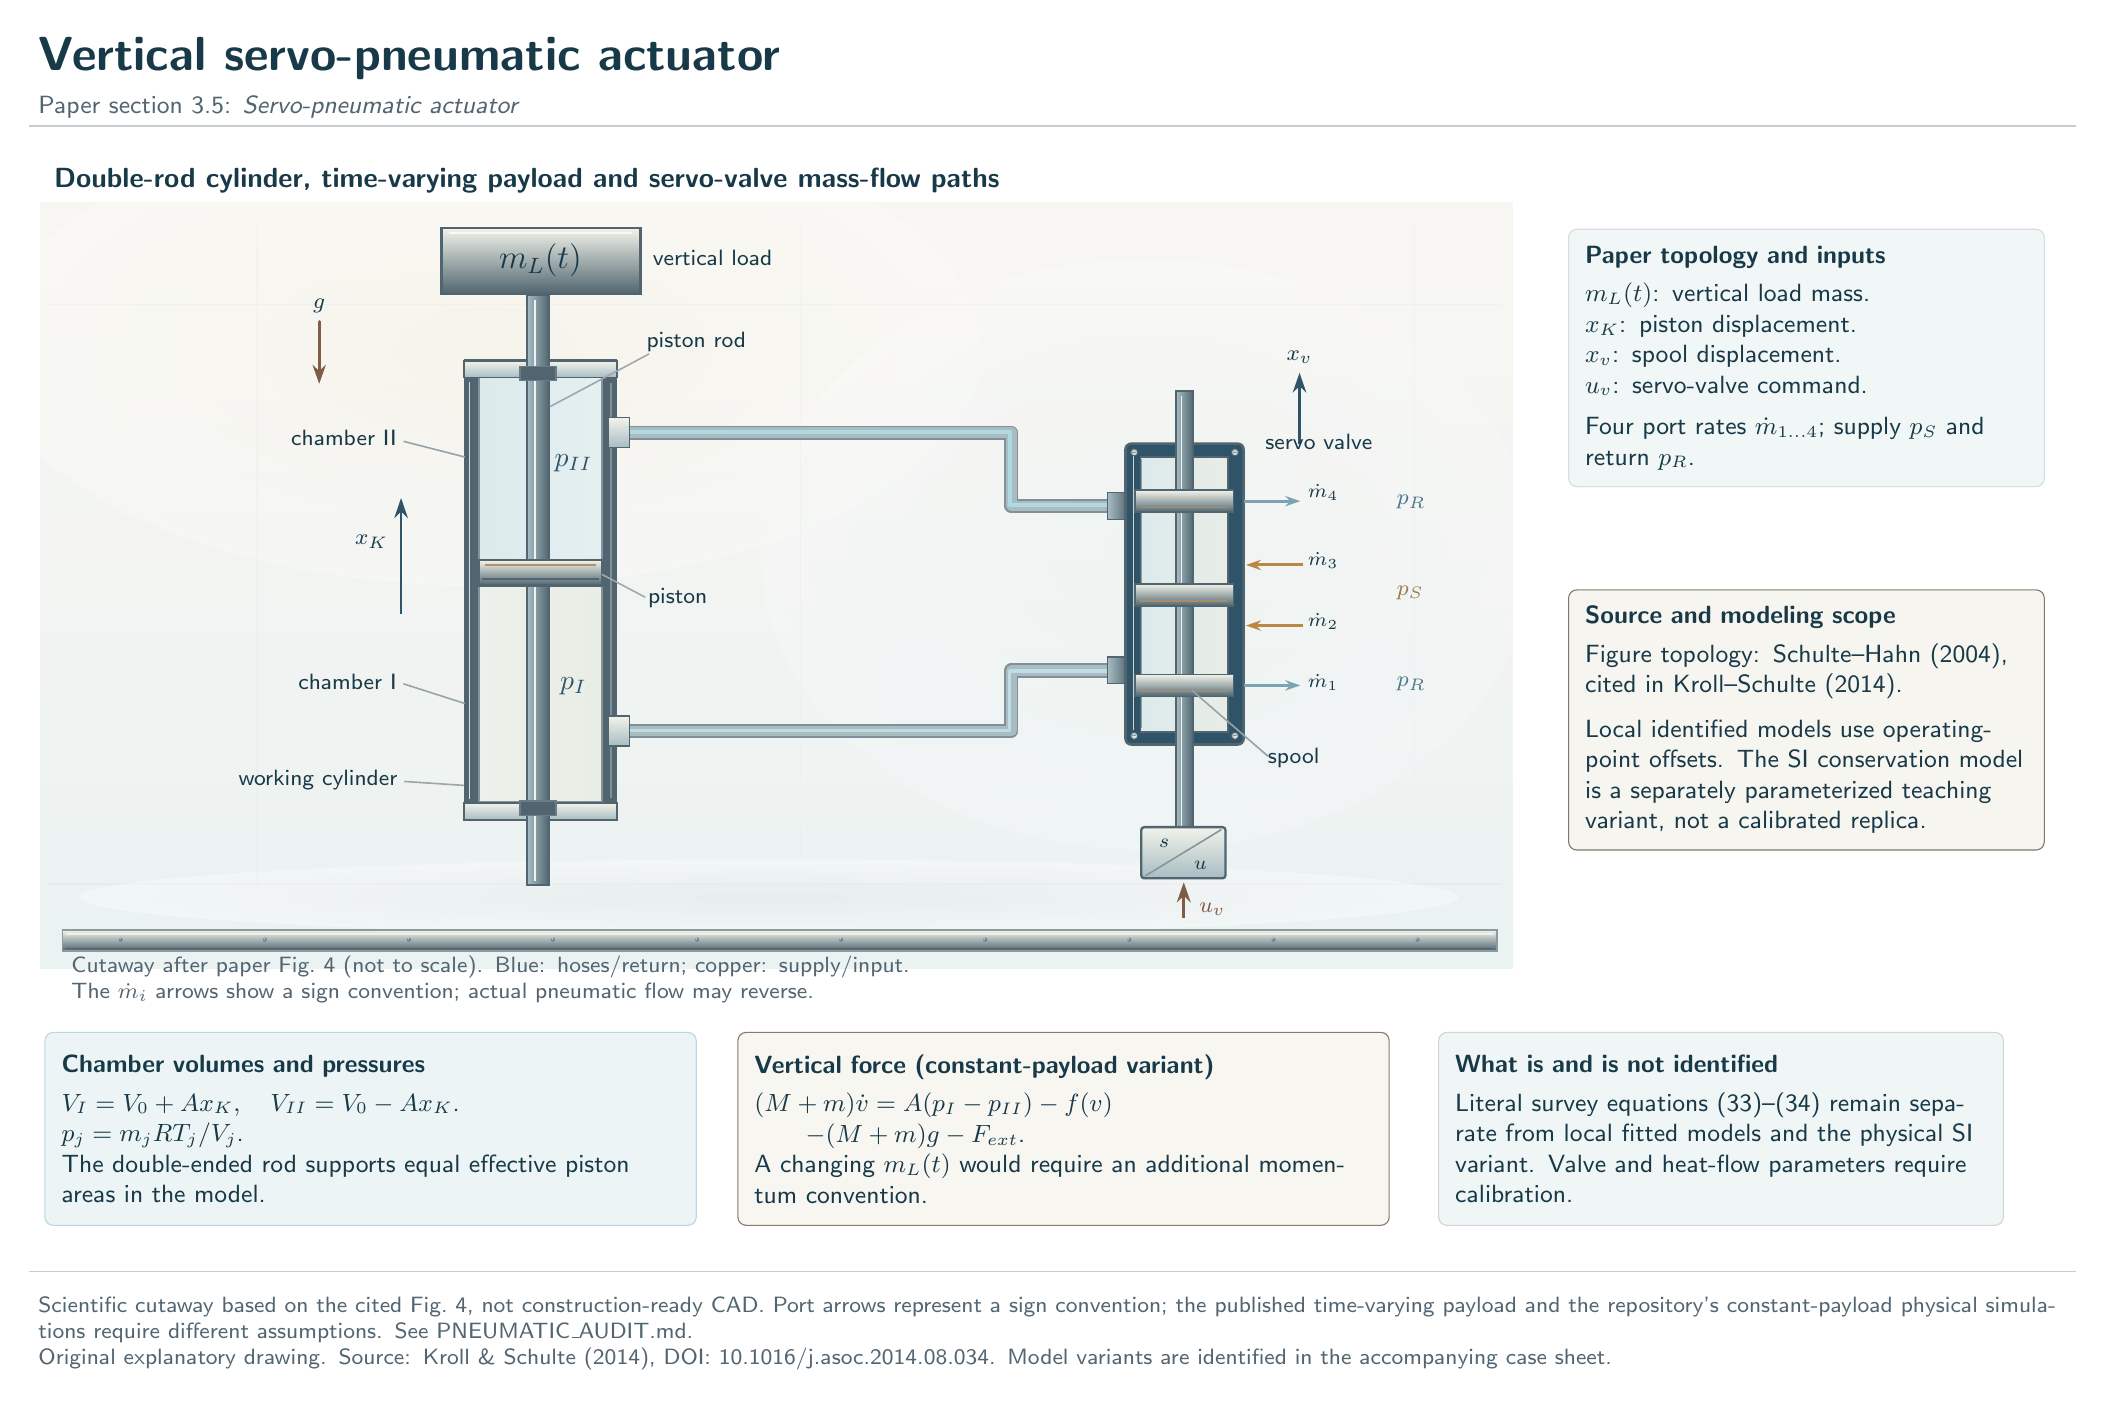
\begin{tikzpicture}[x=1cm,y=1cm]
\atlasheader{Vertical servo-pneumatic actuator}{3.5}{Servo-pneumatic actuator}
\node[anchor=west,font=\sffamily\bfseries] at (.2,-1.95)
 {Double-rod cylinder, time-varying payload and servo-valve mass-flow paths};
% -- LABORATORY CONTEXT -- deliberately subdued, and not a modeled component.
\begin{scope}
 \clip (.14,-2.23) rectangle (18.85,-12.01);
 \shade[top color=wallWarm!77!white,bottom color=wallCool!83!white,opacity=.78]
  (.15,-2.23) rectangle (18.85,-11.96);
 \shade[inner color=dayLight!67!white,outer color=white,opacity=.25]
  (5.8,-4.10) ellipse (6.3cm and 3.0cm);
 \shade[inner color=airLight!30!white,outer color=white,opacity=.18]
  (14.2,-6.70) ellipse (4.9cm and 3.75cm);
 \draw[guide!23,line width=.65pt,opacity=.37]
  (0.25,-10.88)--(18.71,-10.88);
 \draw[guide!19,line width=.55pt,opacity=.30]
  (0.25,-3.52)--(18.71,-3.52);
 \foreach \xx in {2.9,9.8,17.6}{
   \draw[guide!17,line width=.48pt,opacity=.31] (\xx,-2.50)--(\xx,-10.93);
 }
 \shade[inner color=metalMid!37!white,outer color=white,opacity=.35]
  (9.40,-11.05) ellipse (8.75cm and .48cm);
\end{scope}
% Satin aluminum testing platform and isolated supports, without physical claims.
\shade[draw=metalDark!65,line width=.67pt,
 top color=metalLight,middle color=metalMid,bottom color=metalDark]
 (.43,-11.47) rectangle (18.65,-11.73);
\draw[metalLight,line width=.78pt,opacity=.84] (.48,-11.515)--(18.61,-11.515);
\draw[metalDark,line width=.52pt] (.48,-11.70)--(18.60,-11.70);
\foreach \xx in {1.17,3.00,4.83,6.66,8.49,10.32,12.15,13.98,15.81,17.64}{
 \fill[metalDark!80] (\xx,-11.59) circle (.026);
 \fill[white] (\xx-.008,-11.58) circle (.008);
}
% CYLINDER MOUNT: the reference's left-hand vertical double-ended-rod unit.
% It is a sectioned actuator, not a claim of measured steel thickness.
\shade[draw=metalDark,line width=1.18pt,
 left color=metalDark,middle color=metalLight,right color=metalDark]
 (5.55,-4.24) rectangle (7.45,-10.03);
\shade[draw=metalDark!70,line width=.54pt,left color=chamberTwo,
 right color=chamberTwo!75!white]
 (5.72,-4.43) rectangle (7.28,-6.78);
\shade[draw=metalDark!70,line width=.54pt,left color=chamberOne!80!white,
 right color=chamberOne]
 (5.72,-7.09) rectangle (7.28,-9.84);
\shade[draw=metalDark,line width=.68pt,top color=metalLight,bottom color=metalMid]
 (5.53,-4.24) rectangle (7.47,-4.45);
\shade[draw=metalDark,line width=.68pt,top color=metalLight,bottom color=metalMid]
 (5.53,-9.85) rectangle (7.47,-10.07);
% Outer shell bevels maintain vertical parallels and consistent thickness.
\draw[white,line width=.60pt,opacity=.80] (5.60,-4.51)--(5.60,-9.80);
\draw[metalDark!60,line width=.70pt,opacity=.7] (7.40,-4.52)--(7.40,-9.79);
% DOUBLE-ENDED PISTON ROD: continuous from payload to below cylinder.
\shade[draw=metalDark,line width=.68pt,
 left color=metalMid,middle color=metalLight,right color=metalDark]
 (6.33,-3.40) rectangle (6.61,-10.89);
\draw[white,line width=.55pt,opacity=.86] (6.43,-3.46)--(6.43,-10.84);
% Shaft seals mark physical interfaces but do not indicate flow ports.
\foreach \yy in {-4.40,-9.92}{
  \shade[draw=metalDark!85,line width=.52pt,left color=metalDark,
   middle color=metalMid,right color=metalDark]
   (6.24,\yy-.09) rectangle (6.70,\yy+.09);
}
% Piston divides chamber II (above) and chamber I (below).
\shade[draw=metalDark,line width=.83pt,
 top color=metalLight,middle color=metalMid,bottom color=metalDark]
 (5.72,-6.77) rectangle (7.28,-7.09);
\draw[metalDark,line width=.60pt] (5.76,-7.01)--(7.24,-7.01);
\draw[warmBrass!90!metalDark,line width=.90pt] (5.80,-6.83)--(7.20,-6.83);
% Payload/load m_L(t) located on the SAME rod, as in paper Fig. 4.
\shade[draw=metalDark,line width=.95pt,top color=metalLight,
 middle color=metalMid,bottom color=metalDark]
 (5.24,-2.55) rectangle (7.77,-3.39);
\draw[white,line width=.65pt,opacity=.72] (5.34,-2.61)--(7.66,-2.61);
\node[font=\sffamily\bfseries\large,text=ink] at (6.5,-2.96) {$m_L(t)$};
\node[anchor=west,subtlelabel] at (7.92,-2.93) {vertical load};
% Force direction and both displacements (source notation unchanged).
\draw[forcearrow] (3.69,-3.74)--(3.69,-4.53);
\node[anchor=south,subtlelabel] at (3.69,-3.63) {$g$};
\draw[draw=metalDeep,line width=.93pt,-{Stealth[length=2.55mm,width=1.72mm]}]
 (4.73,-7.45)--(4.73,-5.98);
\node[anchor=east,subtlelabel] at (4.57,-6.54) {$x_K$};
% Labels are OPEN text; leaders never touch the source's state labels.
\node[anchor=east,subtlelabel] at (4.68,-5.22) {chamber II};
\draw[guide!73,line width=.58pt] (4.76,-5.26)--(5.54,-5.46);
\node[anchor=east,subtlelabel] at (4.68,-8.31) {chamber I};
\draw[guide!73,line width=.58pt] (4.76,-8.34)--(5.54,-8.59);
\node[anchor=east,subtlelabel] at (4.69,-9.56) {working cylinder};
\draw[guide!72,line width=.58pt] (4.77,-9.58)--(5.53,-9.63);
\node[anchor=west,subtlelabel] at (7.84,-4.00) {piston rod};
\draw[guide!70,line width=.57pt] (7.88,-4.15)--(6.62,-4.82);
\node[anchor=west,subtlelabel] at (7.86,-7.25) {piston};
\draw[guide!70,line width=.57pt] (7.83,-7.24)--(7.28,-6.95);
\node[font=\sffamily\bfseries,text=metalDeep] at (6.92,-5.54) {$p_{II}$};
\node[font=\sffamily\bfseries,text=metalDeep] at (6.92,-8.37) {$p_I$};
% Two distinct continuous pneumatic lines: upper chamber II and lower I.
% Their connection order matches Fig. 4; line colors indicate the chamber,
% not a fixed sign of the reversible servo-valve mass flows.
\draw[metalDark!72,line width=5.15pt,line cap=round,line join=round]
 (7.46,-5.15)--(12.48,-5.15)--(12.48,-6.08)--(13.92,-6.08);
\draw[metalMid,line width=3.75pt,line cap=round,line join=round]
 (7.46,-5.15)--(12.48,-5.15)--(12.48,-6.08)--(13.92,-6.08);
\draw[airLight!80!white,line width=1.33pt,opacity=.84,line cap=round,line join=round]
 (7.48,-5.14)--(12.46,-5.14)--(12.46,-6.07)--(13.88,-6.07);
\draw[metalDark!72,line width=5.15pt,line cap=round,line join=round]
 (7.46,-8.94)--(12.48,-8.94)--(12.48,-8.17)--(13.92,-8.17);
\draw[metalMid,line width=3.75pt,line cap=round,line join=round]
 (7.46,-8.94)--(12.48,-8.94)--(12.48,-8.17)--(13.92,-8.17);
\draw[airLight!65!white,line width=1.25pt,opacity=.83,line cap=round,line join=round]
 (7.48,-8.93)--(12.46,-8.93)--(12.46,-8.18)--(13.88,-8.18);
% Machined cylinder-side fittings and valve couplers.
\foreach \yy in {-5.15,-8.94}{
 \shade[draw=metalDark,line width=.44pt,top color=metalLight,
 bottom color=metalMid] (7.36,\yy-.19) rectangle (7.63,\yy+.19);
}
\foreach \yy in {-6.08,-8.17}{
 \shade[draw=metalDark,line width=.45pt,left color=metalMid,
 middle color=metalLight,right color=metalDark]
 (13.70,\yy-.17) rectangle (13.97,\yy+.17);
}
% SERVO VALVE is to the right, with a genuinely vertical spool as in Fig. 4.
% Brushed deep-blue protective valve casing with a silver center reflection.
\shade[draw=metalDark,line width=.94pt,rounded corners=2.1pt,
 left color=metalDeep,middle color=metalBlue!64!metalLight,right color=metalDeep]
 (13.93,-5.29) rectangle (15.43,-9.11);
\draw[metalLight,line width=.63pt,opacity=.82] (14.03,-5.45)--(14.03,-8.93);
\shade[draw=metalDark,line width=.52pt,left color=chamberTwo,
 middle color=white,right color=chamberOne]
 (14.12,-5.46) rectangle (15.23,-8.95);
\draw[metalDark!64,line width=.46pt] (14.13,-5.49)--(14.13,-8.90);
% Small case screws, subdued to preserve the technical annotation hierarchy.
\foreach \xx/\yy in {14.04/-5.40,15.32/-5.40,14.04/-9.00,15.32/-9.00}{
 \shade[draw=metalDark,line width=.30pt,inner color=metalLight,outer color=metalMid]
  (\xx,\yy) circle (.045);
 \draw[metalDark!68,line width=.27pt] (\xx-.022,\yy)--(\xx+.022,\yy);
}
% Core spool rod: one shaft spans all three lands and the lower drive.
\shade[draw=metalDark,line width=.60pt,left color=metalMid,
 middle color=metalLight,right color=metalDark]
 (14.57,-4.62) rectangle (14.79,-10.42);
\draw[white,line width=.43pt,opacity=.87] (14.64,-4.69)--(14.64,-10.34);
% Three radial land discs and their slim seal edges.
\foreach \yy in {-6.02,-7.21,-8.36}{
 \shade[draw=metalDark,line width=.58pt,top color=metalLight,
 middle color=metalMid,bottom color=metalDark]
 (14.05,\yy-.14) rectangle (15.30,\yy+.14);
 \draw[warmBrass!80!metalDark,line width=.49pt]
 (14.12,\yy-.08)--(15.22,\yy-.08);
}
% Servo spool variable positive upward; explicitly not the piston position.
\draw[metalDeep,line width=1.04pt,-{Stealth[length=2.5mm,width=1.71mm]}]
 (16.14,-5.30)--(16.14,-4.39);
\node[anchor=south,subtlelabel] at (16.14,-4.28) {$x_v$};
\node[anchor=west,subtlelabel] at (15.70,-5.27) {servo valve};
\node[anchor=west,subtlelabel] at (15.73,-9.28) {spool};
\draw[guide!74,line width=.59pt] (15.74,-9.26)--(14.77,-8.42);
% Source Fig. 4 has four signed mass-flow variables, two supply and two
% return locations. These compact horizontal arrows give the source sign
% convention only: pneumatic flow itself may reverse for other spool commands.
\foreach \yy in {-6.02,-8.36}{
 \draw[returnFlow!78,line width=1.03pt,-{Stealth[length=1.9mm,width=1.3mm]}]
 (15.44,\yy)--(16.15,\yy);
}
\foreach \yy in {-6.83,-7.60}{
 \draw[supply,line width=1.07pt,-{Stealth[length=1.9mm,width=1.3mm]}]
 (16.19,\yy)--(15.46,\yy);
}
\node[anchor=west,smalllabel] at (16.24,-5.91) {$\dot m_4$};
\node[anchor=west,smalllabel] at (16.24,-6.77) {$\dot m_3$};
\node[anchor=west,smalllabel] at (16.24,-7.55) {$\dot m_2$};
\node[anchor=west,smalllabel] at (16.24,-8.32) {$\dot m_1$};
\node[anchor=west,subtlelabel,text=returnFlow!78!ink] at (17.37,-6.03) {$p_R$};
\node[anchor=west,subtlelabel,text=supply!82!ink] at (17.37,-7.18) {$p_S$};
\node[anchor=west,subtlelabel,text=returnFlow!78!ink] at (17.37,-8.34) {$p_R$};
% Exposed valve drive, shown as a true s/u symbol, with an upward input.
\shade[draw=metalDark,line width=.85pt,rounded corners=1.1pt,
 top color=metalLight,bottom color=metalMid]
 (14.13,-10.16) rectangle (15.20,-10.81);
\draw[guide!85,line width=.58pt] (14.18,-10.78)--(15.15,-10.19);
\node[font=\sffamily\scriptsize] at (14.42,-10.37) {$s$};
\node[font=\sffamily\scriptsize] at (14.88,-10.64) {$u$};
\draw[draw=copperDeep,line width=1.10pt,-{Stealth[length=2.55mm,width=1.75mm]}]
 (14.67,-11.32)--(14.67,-10.86);
\node[anchor=west,subtlelabel,text=copperDeep] at (14.86,-11.20) {$u_v$};
% A small unboxed provenance cue below the physical instrument.
\node[anchor=west,annotation,text width=18.1cm] at (.42,-12.09)
 {Cutaway after paper Fig.~4 (not to scale). Blue: hoses/return; copper: supply/input.\\
 The $\dot m_i$ arrows show a sign convention; actual pneumatic flow may reverse.};
% -- DOMAIN PANELS: distinguish the original schematic, surveyed models,
% and the separate physical teaching variant without inventing calibration.
\node[labpanel,anchor=north west,text width=5.62cm,align=left]
 at (19.55,-2.56)
 {\textbf{Paper topology and inputs}\\[3pt]
 $m_L(t)$: vertical load mass.\\
 $x_K$: piston displacement.\\
 $x_v$: spool displacement.\\
 $u_v$: servo-valve command.\\[4pt]
 Four port rates $\dot m_{1\ldots 4}$; supply $p_S$ and return $p_R$.};
\node[panel,draw=warmBrass!44!metalDark,fill=wallWarm!70!white,
 anchor=north west,text width=5.62cm,align=left]
 at (19.55,-7.14)
 {\textbf{Source and modeling scope}\\[3pt]
 Figure topology: Schulte--Hahn (2004), cited in Kroll--Schulte (2014).\\[5pt]
 Local identified models use operating-point offsets. The SI conservation model is a separately parameterized teaching variant, not a calibrated replica.};
% -- MODELING PANELS: these are supplemental interpretation, not paper Fig. 4.
\node[panel,draw=airBlue!32,fill=chamberTwo!53!white,
 anchor=north west,text width=7.85cm,minimum height=2.45cm,align=left]
 at (.20,-12.76)
 {\textbf{Chamber volumes and pressures}\\[3pt]
 $V_I=V_0+A x_K,\quad V_{II}=V_0-A x_K$.\\
 $p_j=m_j R T_j/V_j$.\\
 The double-ended rod supports equal effective piston areas in the model.};
\node[panel,draw=warmBrass!48!metalDark,fill=wallWarm!62!white,
 anchor=north west,text width=7.85cm,minimum height=2.45cm,align=left]
 at (9.00,-12.76)
 {\textbf{Vertical force (constant-payload variant)}\\[3pt]
 $(M+m)\dot v=A(p_I-p_{II})-f(v)$\\
 $\qquad -(M+m)g-F_{ext}$.\\
 A changing $m_L(t)$ would require an additional momentum convention.};
\node[panel,draw=metalDark!27,fill=wallCool!47!white,
 anchor=north west,text width=6.75cm,minimum height=2.45cm,align=left]
 at (17.90,-12.76)
 {\textbf{What is and is not identified}\\[3pt]
 Literal survey equations (33)--(34) remain separate from local fitted models and the physical SI variant. Valve and heat-flow parameters require calibration.};
\atlasfooter{Scientific cutaway based on the cited Fig.~4, not construction-ready CAD. Port arrows represent a sign convention; the published time-varying payload and the repository's constant-payload physical simulations require different assumptions. See PNEUMATIC\_AUDIT.md.}
\end{tikzpicture}
\end{document}
